\documentclass[report]{jsbook}
\usepackage[dvipdfmx]{graphicx}
\usepackage[dvipdfmx]{color}
\usepackage{okumacro}
\usepackage{fancybox,ascmac}
\usepackage{sty/algorithm}
\usepackage{sty/algorithmic}
\usepackage{colortbl}
\usepackage{multirow}
\usepackage{listings}
\usepackage{sty/jlisting}
\usepackage{url}
\usepackage{color}
\usepackage[noreplace]{otf}
\usepackage{comment}

\lstset{
	language={Java},
	basicstyle={\small},
	breaklines={true},
	frame=tRBl,
	framesep=5pt,
}

\usepackage{url}

\setcounter{tocdepth}{2}

%%%%%%%%%%


%%%%%%%%%%%%%%%%%%

\begin{document}
\pagestyle{empty}

\begin{center}

\vspace{5cm}

\textbf{\Large 卒業論文~2020年度(令和2年度)}

\vspace{2cm}

\textbf{\LARGE ADLogger: 朝のタスク別時間記録システム}

\vspace{3cm}

\textbf{\underline{\large 指導教員}}\\
\textbf{慶應義塾大学環境情報学部}

\textbf{\Large 中澤~~仁}\\
\textbf{\Large 矢作~~尚久}\\
\textbf{\Large 村井~~純}\\
\textbf{\Large 楠本~~博之}\\
\textbf{\Large 中村~~修}\\
\textbf{\Large 高汐~~一紀}\\
\textbf{\Large Rodney D. Van Meter III}\\
\textbf{\Large 植原~~啓介}\\
\textbf{\Large 三次~~仁}\\
\textbf{\Large 武田~~圭史}\\

\vspace{6cm}

\textbf{\LARGE 慶應義塾大学 環境情報学部}

\vspace{.5em}

\textbf{\LARGE 助川 友理}

\vspace{.3em}

\textbf{\it suke@ht.sfc.keio.ac.jp}



\newpage

\end{center}

\pagestyle{plain}

\frontmatter
\begin{center}
\textbf{\Large 卒業論文要旨 2020年度(令和2年度)}

\vspace{6.18mm}

\textbf{\Large ADLogger: 日常生活動作の為のタスク別時間記録システム}
\end{center}

\vspace{10mm}

\begin{flushleft}
\textbf{論文要旨}\\
\end{flushleft}
今日私達の生活において,時間管理は欠かせないものになっている.
一方で個人管理としての時間管理はまだ進んでいるとは言い難い.
本研究は正確な行動時間把握を目的とするiOSアプリケーションを提案し,時間管理行動に対する苦手意識や行動の変化を与える事を目的とする.
具体的には実測値の記録及び三点見積もり法を用いた自動計算機能が搭載した.後できちんと書く.




\begin{flushleft}
\textbf{キーワード}\\
\textbf{時間知覚(認知),遅刻,行動変容,メタ認知,心理的時間,Well-being Computing}

\end{flushleft}

\begin{flushright}
\textbf{慶應義塾大学 環境情報学部}\\
\textbf{助川 友理}
\end{flushright}
\newpage



\setlength{\baselineskip}{13pt}
\begin{center}
\textbf{\large Abstract of Bachelor's Thesis Academic Year 2020}

\vspace{6mm}

\textbf{\large ADLogger:Behavior Modification for ADL Time Management}
\end{center}

\vspace{10mm}


\begin{flushleft}
\textbf{Abstract}\\
\end{flushleft}

Time management needs expect time for task and buffer correctly. “ADLogger” is the system that expect how much time you may spend to the task and define the accurate buffer according to your time log data. The research will evaluate the accuracy of subjects’ time prediction, and comparing subjects’ behavior before and after using the system.
日本語の概要欄を書き終え次第執筆する.

\begin{flushleft}
\textbf{Keywords}\\
\textbf{Well-being Computing}
\end{flushleft}

\begin{flushright}
\textbf{Keio University Faculty of Environment and Information Studies}\\
\textbf{Yuri Sukegawa}\\
\end{flushright}

\setlength{\baselineskip}{16pt}
\tableofcontents
\listoffigures
\listoftables

\mainmatter
\chapter{序論}
本章では,はじめに本研究における背景を述べる.
ついで,問題意識および本研究の目的を述べる.
最後に本論文の構成を示す.

\section{背景}

私たちは長きに渡って時間を客観的種票として共同生活を続けている\cite{history}.
近年では時間を資源として考え,時間管理を心がける場面は公私双方様々な場面で存在する.
特にプロジェクト管理においては「感覚に依存した見積もりの誤差」「バッファの不備」による計画の失敗を非常に懸念する\cite{innopm}.
その為プロジェクト管理に対する計画においては時間管理を非常に重要なものであると位置付ける事が多く,これまで多くのフレームワークが考案されている.
一方で個人管理としての時間管理はまだ進んでいるとは言い難い.
例えば文京学院大学による遅刻の状況の調査によると授業・友達の待ち合わせ共に「逆算の甘さ」が一因となり遅刻すると考えている人が多数を占める\cite{bunkyo}.

\section{目的}
本研究は個人管理における時間管理の失敗に関する仮説を提案した上で,
行動時間の実測値記録及び必要時間の簡算出機能を搭載したiOSアプリケーションを提案し,時間管理行動に変化を与える事を目的としている.

\section{構成}
本論文は,本章を含め全8章からなる.
本章では,本研究における背景と目的を述べた.
第2章では,関連研究を整理する.
第3章では,これまでに開発してきたシステムとその評価結果について説明し,本研究における問題意識について述べる.
第4章では,本研究における要件を述べ,本研究で提案するシステムの概要について説明する.
第5章では,本システムの設計について述べる.
第6章では,本システムの実装について説明する.
第7章では,本システムで得られたデータから評価を行い,考察について述べる.
第8章では,本論文の結論と今後の展望について整理する.
\chapter{関連研究}
関連研究や用語の定義,先行研究及びアプリケーションの先行事例を示す.

\section{時間管理の定義}
時間管理の定義はまだ明確に定まっていない.
例えば著名なものとしてLakeinの定義\cite{Lakein1989}の定義が挙げられる(表~\ref{tb:Lakein}).
Lakeinは個人管理という位置付けで時間管理に言及し,下記の4項目に則り時間管理を遂行していく重要性を説いた.

\begin{table}[htb]
\begin{center}
  \begin{tabular}{|l|l|} \hline
   1 & すべきことを決定する \\ \hline
   2 & 達成するための目標を設定する \\ \hline
   3 & 優先順位を決める \\ \hline
   4 & 取り組む課題のプランニングを作る \\ \hline
  \end{tabular}
  \caption{Lakeinによる時間管理の定義}
  \label{tb:Lakein}
\end{center}
\end{table}

Claessens et al. は,先行研究の定義を俯瞰した上で,時間管理を"目標を達成するために時間を効果的に使用する行動"と定義し時間管理の行動を更に以下の3つに分類した\cite{Claessens2007}(表 ~\ref{tb:Claessens}).

\begin{table}[htb]
\begin{center}
  \begin{tabular}{|l|l|} \hline
   時間アセスメント行動(time assessment behavior): \\ ~~~過去,現在,未来の時間を認識し,時間の使い方に関して認識する事 \\ \hline
   プランニング行動(planning behavior): \\  ~~~時間を効率的に使用する事を目的とする事 \\ \hline
   モニタリング行動(monitoring behavior): \\ ~~~行動中における時間の配分のモニタリング・不測の事態へのリスクヘッジ等 \\ \hline
  \end{tabular}
  \caption{Claessens et al. による時間管理の定義}
  \label{tb:Claessens}
\end{center}
\end{table}

\section{時間管理の先行研究について}
時間管理研究は大きく分けて時間管理がもたらす効果の研究と時間管理能力に関する研究の2種類に分けられる.
前者は更に以下の3つに分類が可能である(表~\ref{tb:senko}).
\begin{table}[htb]
\begin{center}
  \begin{tabular}{|l|l|} \hline
   1 & 時間管理と他の指標の相関関係を調べる研究 \\ \hline
   2 & 時間管理のプロセスモデルの研究 \\ \hline
   3 & 時間管理トレーニングの研究 \\ \hline
  \end{tabular}
  \caption{時間管理がもたらす効果の研究の概要}
  \label{tb:senko}
\end{center}
\end{table}

後者の時間管理能力の研究では必要時間の正確な見積もりの能力に関する研究である.
時間管理能力に関しては主に見積もり時間の精度に関して議論されている.
見積もりの精度は大きく分けて課題に対するもの\footnote{与えられた課題の時間 \cite{Roy2008}や経験の有無\cite{Roy2007}}と被験者の個人差によるもの\footnote{時間評価における知覚時間の歪み\cite{Oguro1961}\cite{Murakami2016}}の2種類存在しているが,
原因として記憶との関連性が考えられている\cite{Roy2005}.

正確な見積もりを計算する手法は主に大規模プロジェクト向けに提案される事が多い.
例えばPERT(Program Evaluation and Review Technique)では個々のタスクの見積もりを予測する手法である「三点見積もり法」が考案されている.
タスク完了に要する時間の最良見積もり(期待時間)値を$T_{E}$,タスク完了に必要な最小時間の予測(楽観的時間)を$O$,タスク完了に必要と思われる最頻値の見積時間(最確時間)を$M$,タスク完了に必要な最大時間の予測(悲観的時間)を$P$とすると,数式(\ref{pert})の様に見積もりを行う\footnote{ただし,三点見積もり法は参加者が複数人いる長期の大型プロジェクトに対する適切な管理方法であり,参加者の多くないプロジェクトでは最可能値だけを使用した見積りのほうが正確である場合がある\cite{Kato1965}}.
\begin{equation}
\label{pert}
T_{E} = (O + 4M + P) ÷ 6
\end{equation}

\section{時間管理の評価方法}
代表的な時間評価の方法としては,被験者に時間の長さを教示し,その長さを産生させる時間産生法(時間作成法)(time production),
被験者が時間を経験した後に体験時間を再生させる時間再生法(time reproduction),
経過した時間間隔を言語的に評価する言語的時間評価法(verbal timeestimation)などがある\cite{Oguro1961}\cite{Tayama2018}.

\section{日常生活動作、及び個人管理としての時間管理}
日常生活動作(Activities of Daily Living;ADL)とは,人が日常生活において繰り返す,身の回りの活動や動作のことである.具体的には,身の回りの動作(食事,更衣,整容,排泄,入浴の各動作),移動動作,その他生活関連動作(家事動作,交通機関の利用等)を指す\cite{Sakai2003}.
今日では特にパフォーマンスやストレスなど様々な観点から個人管理面においても適切な時間管理が求められている.\cite{Barling1996}\cite{Britton1991}\cite{Burt1994}\cite{Macan1994}.

\section{時間管理をサポートするシステム}
今日,日常生活動作を基調とし,身近な時間管理をサポートするシステムが複数開発されている.私は現在開発されたアプリケーションの種類を以下の3種類に分類した(表 ~\ref{tb:app}).

\begin{table}[htb]
\begin{center}
  \begin{tabular}{|l|l|} \hline
   1 & タイムログ \\ \hline
   2 & ルーチン補助 \\ \hline
   3 & ストップウォッチ \\ \hline
  \end{tabular}
  \caption{時間管理ツールの分類}
  \label{tb:app}
\end{center}
\end{table}

1つ目のタイムログに関しては日毎のタスクをなるべく多く記録・計測を行い,一日の時間の使い方を可視化する事を目的としているものである.
このシステムの先行事例には たすくま\cite{Taskuma} や toggl\cite{toggl} (図~\ref{fig:toggl})が挙げられる.
\\
\begin{figure}[ht]
\begin{center}
\begin{tabular}{c}

  	\begin{minipage}[b]{0.5\linewidth}
	\begin{center}
		\fbox{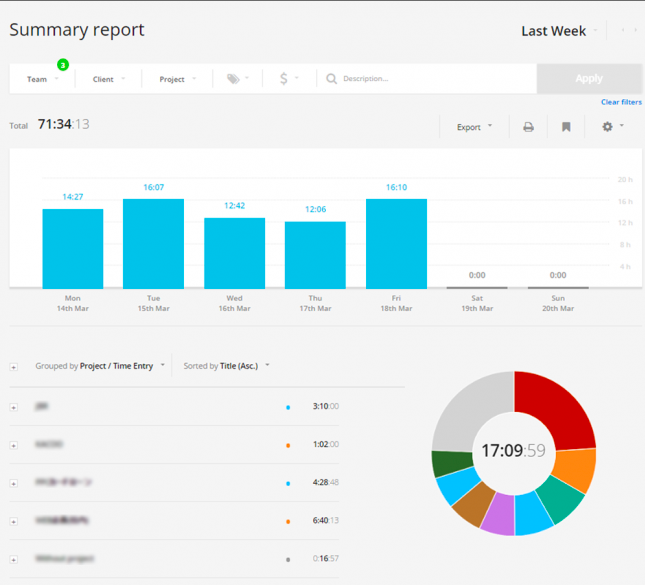
\includegraphics[width=10cm]{images/2/toggl.png}}
		\caption{togglによるログの可視化}
		\label{fig:toggl}
	\end{center}
  	\end{minipage}
\end{tabular}
\end{center}
\end{figure}
\\

2つ目のルーチン補助に関しては,自分がこれから行いたいルーチンをリマインド音などを用いてコントロールするものである.
このシステムの先行事例には自分でやる事を設定する ルーチンタイマー\cite{RoutineTimer} (図~\ref{fig:routine})やポモドーロテクニック\cite{pomodoro} に則ったリマインドアプリなどがある.
\\
\begin{figure}[ht]
\begin{center}
\begin{tabular}{c}

  	\begin{minipage}[b]{0.5\linewidth}
	\begin{center}
		\fbox{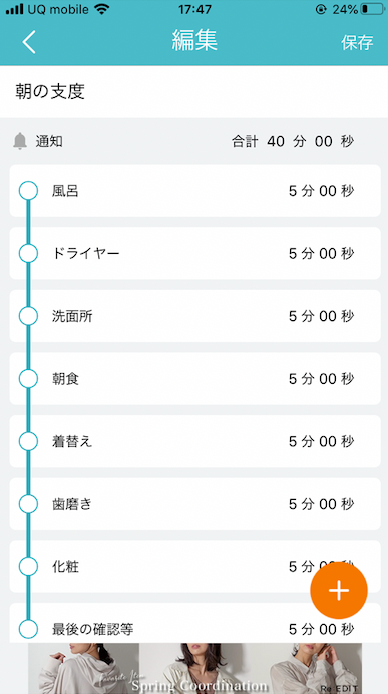
\includegraphics[width=5cm]{images/2/routine.png}}
		\caption{ルーチンタイマーの行動設定例}
		\label{fig:routine}
	\end{center}
  	\end{minipage}
\end{tabular}
\end{center}
\end{figure}
\\
3つ目のストップウォッチに関しては,ストップウォッチを主機能として時間把握に役立てようとするものであり,用途・目的は様々である.
例えば時間の流れをイラストで表現するもの(ねずみタイマー\cite{MouseTimer}(図~\ref{fig:mouse}))や時間把握の精度をミニゲームに昇華させたもの\cite{JUSTTIME},ストップウォッチとメモ帳を組み合わせたもの\cite{StopNote}などが挙げられる.
\begin{figure}[ht]
\begin{center}
\begin{tabular}{c}

  	\begin{minipage}[b]{0.5\linewidth}
	\begin{center}
		\fbox{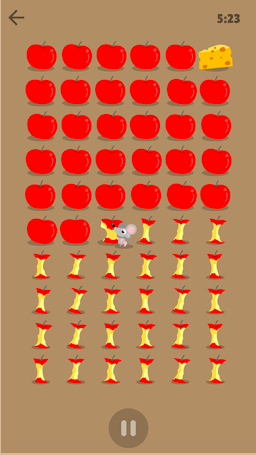
\includegraphics[width=5cm]{images/2/mouse.png}}
		\caption{ねずみタイマーによる経過時間の可視化}
		\label{fig:mouse}
	\end{center}
  	\end{minipage}
\end{tabular}
\end{center}
\end{figure}

\section{まとめ}
本章では,本研究における関連研究を整理し,問題意識を洗い出した.
次章では,筆者が本研究に先立ち行った研究について述べ,問題意識を洗い出す.
\section{先行研究からの問題意識}
学術面として最適な見積もりを考える手法は大規模なプロジェクト向けのものが多く,日常生活動作向けに個人管理として使えるものか十分な検証はなされていない.
特に時間評価は日常生活動作を評価する30分から60分規模の研究が乏しい上,見積もりの誤差が小さくなればどういう効果が現れるかに対して検証する研究はなされていない.
またアプリケーションにおいても図~\ref{fig:bottomup}が示す様に短期間における自分の時間傾向を予測する(未来型)のものは無い.

\section{予備実験}
\subsection{予備実験の概要}
本研究に先立ち,時間の逆算の甘さという現象を実測で分析する予備実験を慶應義塾大学大学生20代男女9人を対象に7日間行った.
まず,被験者にインタビューを行い,時間管理に対し苦手意識があるグループと無いグループの2つにグループ分けを行った.今回9人中6人の被験者は朝の時間管理に対し苦手意識があると答えた.次に,遂行タスクをtodoリスト形式で事前登録を行ってもらった上で図~\ref{tb:Q}の項目を被験日時までに被験者に予想して貰った.また,総所要予測時間1 を $T_{1}$,総所要予測時間2 を$T_{2}$,理想の外出時刻を$I$,外出時刻のタイムリミットを$L$,支度開始時刻を$B$と置いた時の数式\ref{1}及び数式\ref{2}を用いて被験者に対する質問項目から必要時間の予測を行った.最後に,タスク別記録アプリケーションを用いて朝の外出準備行動に関するタスク毎の必要時間予測と実測の比較を行った.タスク別記録アプリケーションは予備実験の為に作成されたiOSアプリケーションである.TODOリスト形式でのタスク名登録,タスクの総時間計測,カラム毎のストップウォッチを用いた各タスクの経過時間の記録が可能である.(表~\ref{fig:yobiapp}参照)

\begin{equation}
\label{1}
 T_{1} = I - B 
\end{equation}

\begin{equation}
\label{2}
 T_{2} = L - B
\end{equation}

\begin{figure}[ht]
\begin{center}
\begin{tabular}{c}

	\begin{minipage}[b]{0.5\linewidth}
	\begin{center}
		\fbox{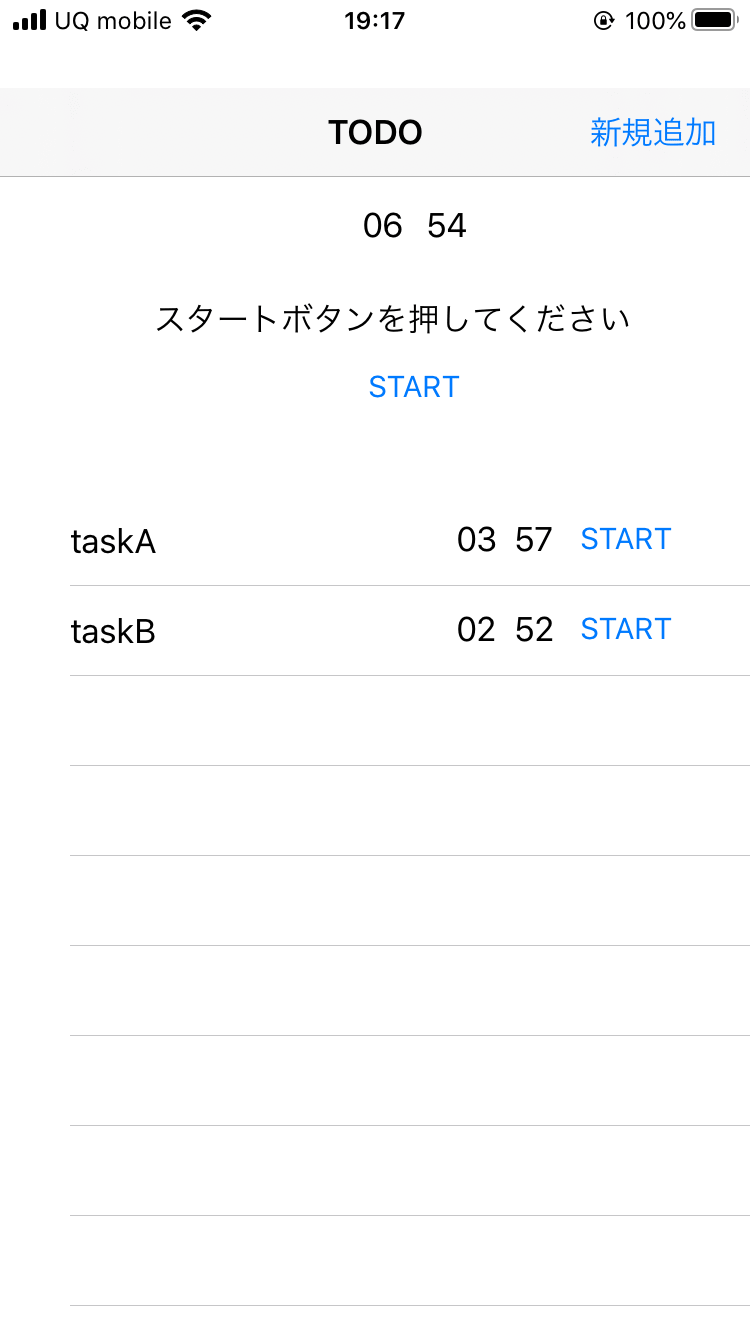
\includegraphics[width=5cm]{images/3/yobi.png}}
		\caption{使用アプリケーション}
		\label{fig:yobiapp}
	\end{center}
  	\end{minipage}
	
\end{tabular}
\end{center}
\end{figure}

\begin{table}[htb]
\begin{center}
  \caption{被験者に対する質問項目}
  \begin{tabular}{|l|l|} \hline
   1 & 支度開始時刻 \\ \hline
   2 & 外出時刻 (理想時刻,外出時刻のタイムリミット) \\ \hline
   3 & 必要タスク \\ \hline
   4 & タスク別所要時間 \\ \hline
  \end{tabular}
  \label{tb:Q}
\end{center}
\end{table}

\subsection{実験結果}
計測日数が0日だった6名(内時間管理に苦手意識のある被験者は5名)を分析対象から除外し,
有効回答者3名(内時間管理に苦手意識のある被験者は1名)を分析の対象とした.
以後被験者A,B,C,と供述する.被験者データとしては被験者Aのみ苦手意識があり.被験者Bのみ3日間,それ以外が1日間のデータが得られた.
図~\ref{fig:re1},\ref{fig:re2}は横軸を被験者名,縦軸を予測時間と実際の時間の差分を可視化したものである.
日常生活動作において被験者A,B,Cは最大3分以上認識の誤差が生じていた.両者グループを比較した際は,Aの方がより誤差の範囲が大きかった.
\begin{figure}[ht]
\begin{center}
\begin{tabular}{c}

	\begin{minipage}[b]{0.5\linewidth}
	\begin{center}
		\fbox{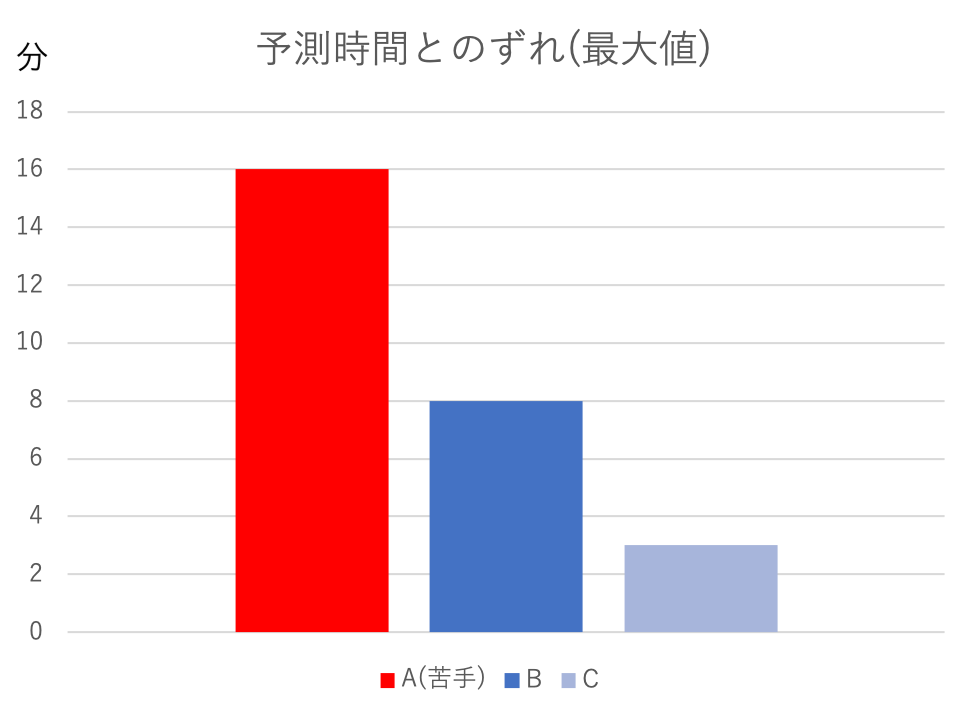
\includegraphics[width=8cm]{images/3/1.png}}
		\caption{被験者結果(最大値)}
		\label{fig:re1}
	\end{center}
  	\end{minipage}
	
		\begin{minipage}[b]{0.5\linewidth}
	\begin{center}
		\fbox{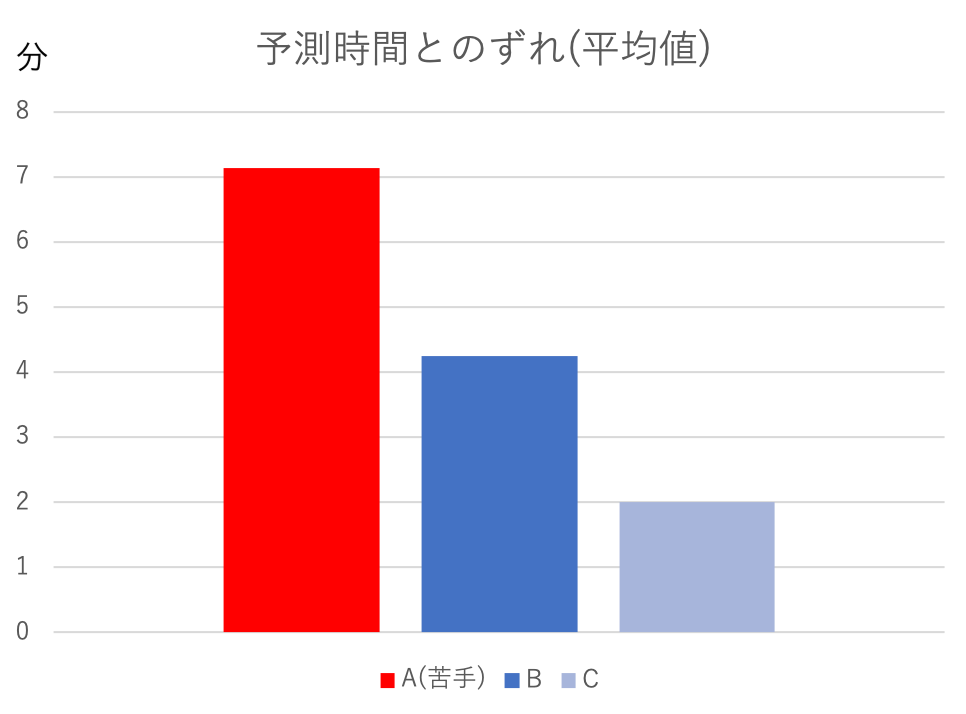
\includegraphics[width=8cm]{images/3/2.png}}
		\caption{被験者結果2}
		\label{fig:re2}
	\end{center}
  	\end{minipage}

\end{tabular}
\end{center}
\end{figure}

また,被験者によっては時間の計画の時点から不備が発生している日もあった.Bにおいては日常生活動作毎の予測時間の合計が予想準備時間(支度開始見込み時刻 - 第一理想時刻)を超えており,計画面から間に合わない計画を立てていた.(事実その日は第一理想時刻には間に合わず,第一理想時刻と第二理想時刻の間に外出していた.)また,それぞれの日常生活動作の内訳は以下の通りである.

\begin{figure}[hb]
	\begin{center}
	\fbox{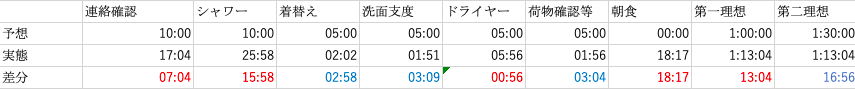
\includegraphics[width=12cm]{images/3/A.png}}
		\caption{被験者Aの内訳}
		\label{fig:top_point}
	\end{center}
\end{figure}

\begin{figure}[hb]
	\begin{center}
	\fbox{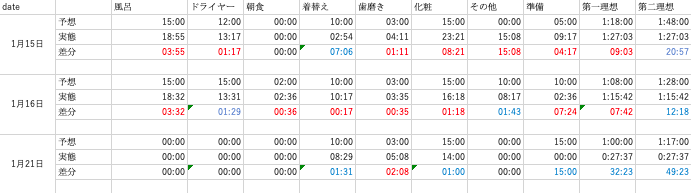
\includegraphics[width=12cm]{images/3/B.png}}
		\caption{被験者Bの内訳}
		\label{fig:top_point}
	\end{center}
\end{figure}

\begin{figure}[hb]
	\begin{center}
	\fbox{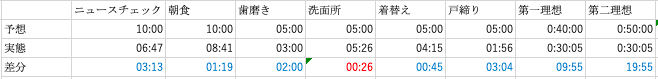
\includegraphics[width=12cm]{images/3/C.png}}
		\caption{被験者Cの内訳}
		\label{fig:top_point}
	\end{center}
\end{figure}

\section{狙い}
3.2で行った実験の結果から,「逆算が苦手」の定義は複数人規模のプロジェクト管理でも言及されていた事と同様に,各タスク見込み時間を実態より短く認識している「見積もり時間の誤差の大きさ」場合とタスク見込み時間の総時間と総準備時間の認識が合致していない上に不十分な予備時間の確保である「バッファの不備」が原因である場合が考えられる.更に破綻したデータは苦手意識のないグループで発見された為,本人の苦手意識にか関わらず被験者の時間管理能力を把握していく必要があると考えられる.
一方で,本予備実験においては被験者数・有効データ数共に少なく,更なる実験が必要であると考えられる.

本研究では,「逆算が苦手」の定義をデータを用いて更なる分析を進めると共に,主要な原因であると考えられる時間管理の見積もり精度に起因された逆算の甘さをiOSアプリケーションを用いて補正する事で時間管理に関する心理的負荷及び逆算精度の改善を図る.
\chapter{システム}
本章では,日常生活動作別の時間記録アプリケーション,ADLoggerを提案する.
はじめにADLoggerシステムの概要を述べ,次にADLoggerの特徴を説明する.
そして最後に,ユーザがADLoggerを利用する流れについて述べる.

\section{ADLoggerシステムの概要}
ADLoggerは行動名別に経過時間を記録するiOSアプリケーションである.
予測算出画面では,行動別の平均時間がリスト形式でカラム毎に出力される.
また,カラムを複数選択する事で複数行動を行う際の必要時間を計算・可視化する事が可能である.

\section{ADLoggerシステムの特徴}
本節では,ADLoggerシステムの特徴としてあげられる機能を挙げる.
\subsection{タスク別ストップウォッチ記録}
簡単な操作で行動名毎に行動時間を記録される.
\subsection{各時間予測}
各行動を下記の計算方法を用いて記録時間の標準的な時間を算出し,リスト形式で行動別に表示する.
\subsection{合計時間の算出}
リストのカラムをタップすると,選択された行動の合計の必要時間を下記の計算手法を元に算出する.
\section{平均時間の算出方法}
\subsection{各時間予測}

\subsection{合計時間の算出}

%これからきちんと書こう



\section{ADLoggerシステムの使用方法}
本アプリケーションを開くと,ログイン認証後図の様なトップ画面が開かれる.%~\ref{fig:top}

ユーザはまず,トップ画面にある``TIMER"ボタンにより,行動を記録する.
``TIMER"ボタンを押すと,``START"ボタンのあるストップウォッチ画面が現れる.
``START"ボタンを押すとストップウォッチが起動し時間を計測できる.
計測後は``STOP"ボタンを押す.出力されるアラートの中から``終了"ボタンを選択し,タスク名選択画面に移行する.
尚,記録を破棄したい場合はアラートの``Reset"ボタンを,ストップウォッチを止めたくない場合は`計測に戻る"を選択する.

タスク選択画面では行動名がリスト形式で表示されている.一度でも登録された行動名であれば行動名を選択する事で経過時間を保存する事ができる.
新たな行動名であれば``新規追加"ボタンを押し,出力されたアラートに行動名を入力し名前を登録後上記同様に保存する.

一度でも記録時間が保存されると``ADLog"ボタンから行動記録を見る事が可能である.
ユーザは必要に応じてタスクを選択しする事で,複数タスクの合計時間を見る事が可能である.

また,利用規約,実験の説明,アプリの使用方法などはアプリケーションを開いた先にある``HELP"ボタンから確認が可能な様にする.

\begin{comment}
記録には,実際に測定する方法と手動で入力する方法の2種類がある.
実際に測定する方法を選択した場合には,ストップウォッチのようにして学習時間を測定する.
測定中の画面を図~\ref{fig:measure4}に示す.

1件でも学習記録が保存されると,図~\ref{fig:outline4}のようにトップ画面に学習記録の概要が表示されるようになる.
ユーザは日ごとや週ごとの学習時間を棒グラフで,学習した教科や内容の割合を円グラフで閲覧することができる.
また,学習を記録した日が色付けされたカレンダーも生成される.

週に一度,動機づけに関するアンケートがユーザに対して実施される.
アンケート回答画面を~\ref{fig:questionnaire4}に示す.
このアンケートによりユーザの動機づけタイプが測定され,その結果に応じてトップ画面に表示される機能が切り替わる.
ポイント機能では学習時間に応じた獲得ポイントが,ランキング機能は他ユーザも合わせた総学習時間のランキングが表示される.
目標設定機能の場合は,はじめにユーザはその週の目標学習時間を設定するよう指示される.
以後は目標に対する達成割合が表示される.
\end{comment}

\section{まとめ}
本章では,日常生活動作別行動時間記録及びリマインドを目的としたADLoggerシステムを提案した.
また,ADLoggerシステムの特徴および使用方法を述べた.
次章では,本システムの設計について述べる.
\section{本システムの設計概要}
本研究では,行動別時間を可視化し,必要時間を簡単に算出させるため,ADLoggerシステムを提案する.
ADLoggerは行動時間を記録し,記録された時間を元にタスク別に必要時間を予測するiOSアプリケーションである.
クライアント側はタスク別時間記録モジュール,必要時間予測モジュール,カレンダー登録モジュール,アンケートモジュール,バッファ制御モジュール,表示制御モジュールから成る.
サーバ側ではデータベースへの書き込み及び読み込みを行う.

\begin{figure}[tb]
	\begin{center}
	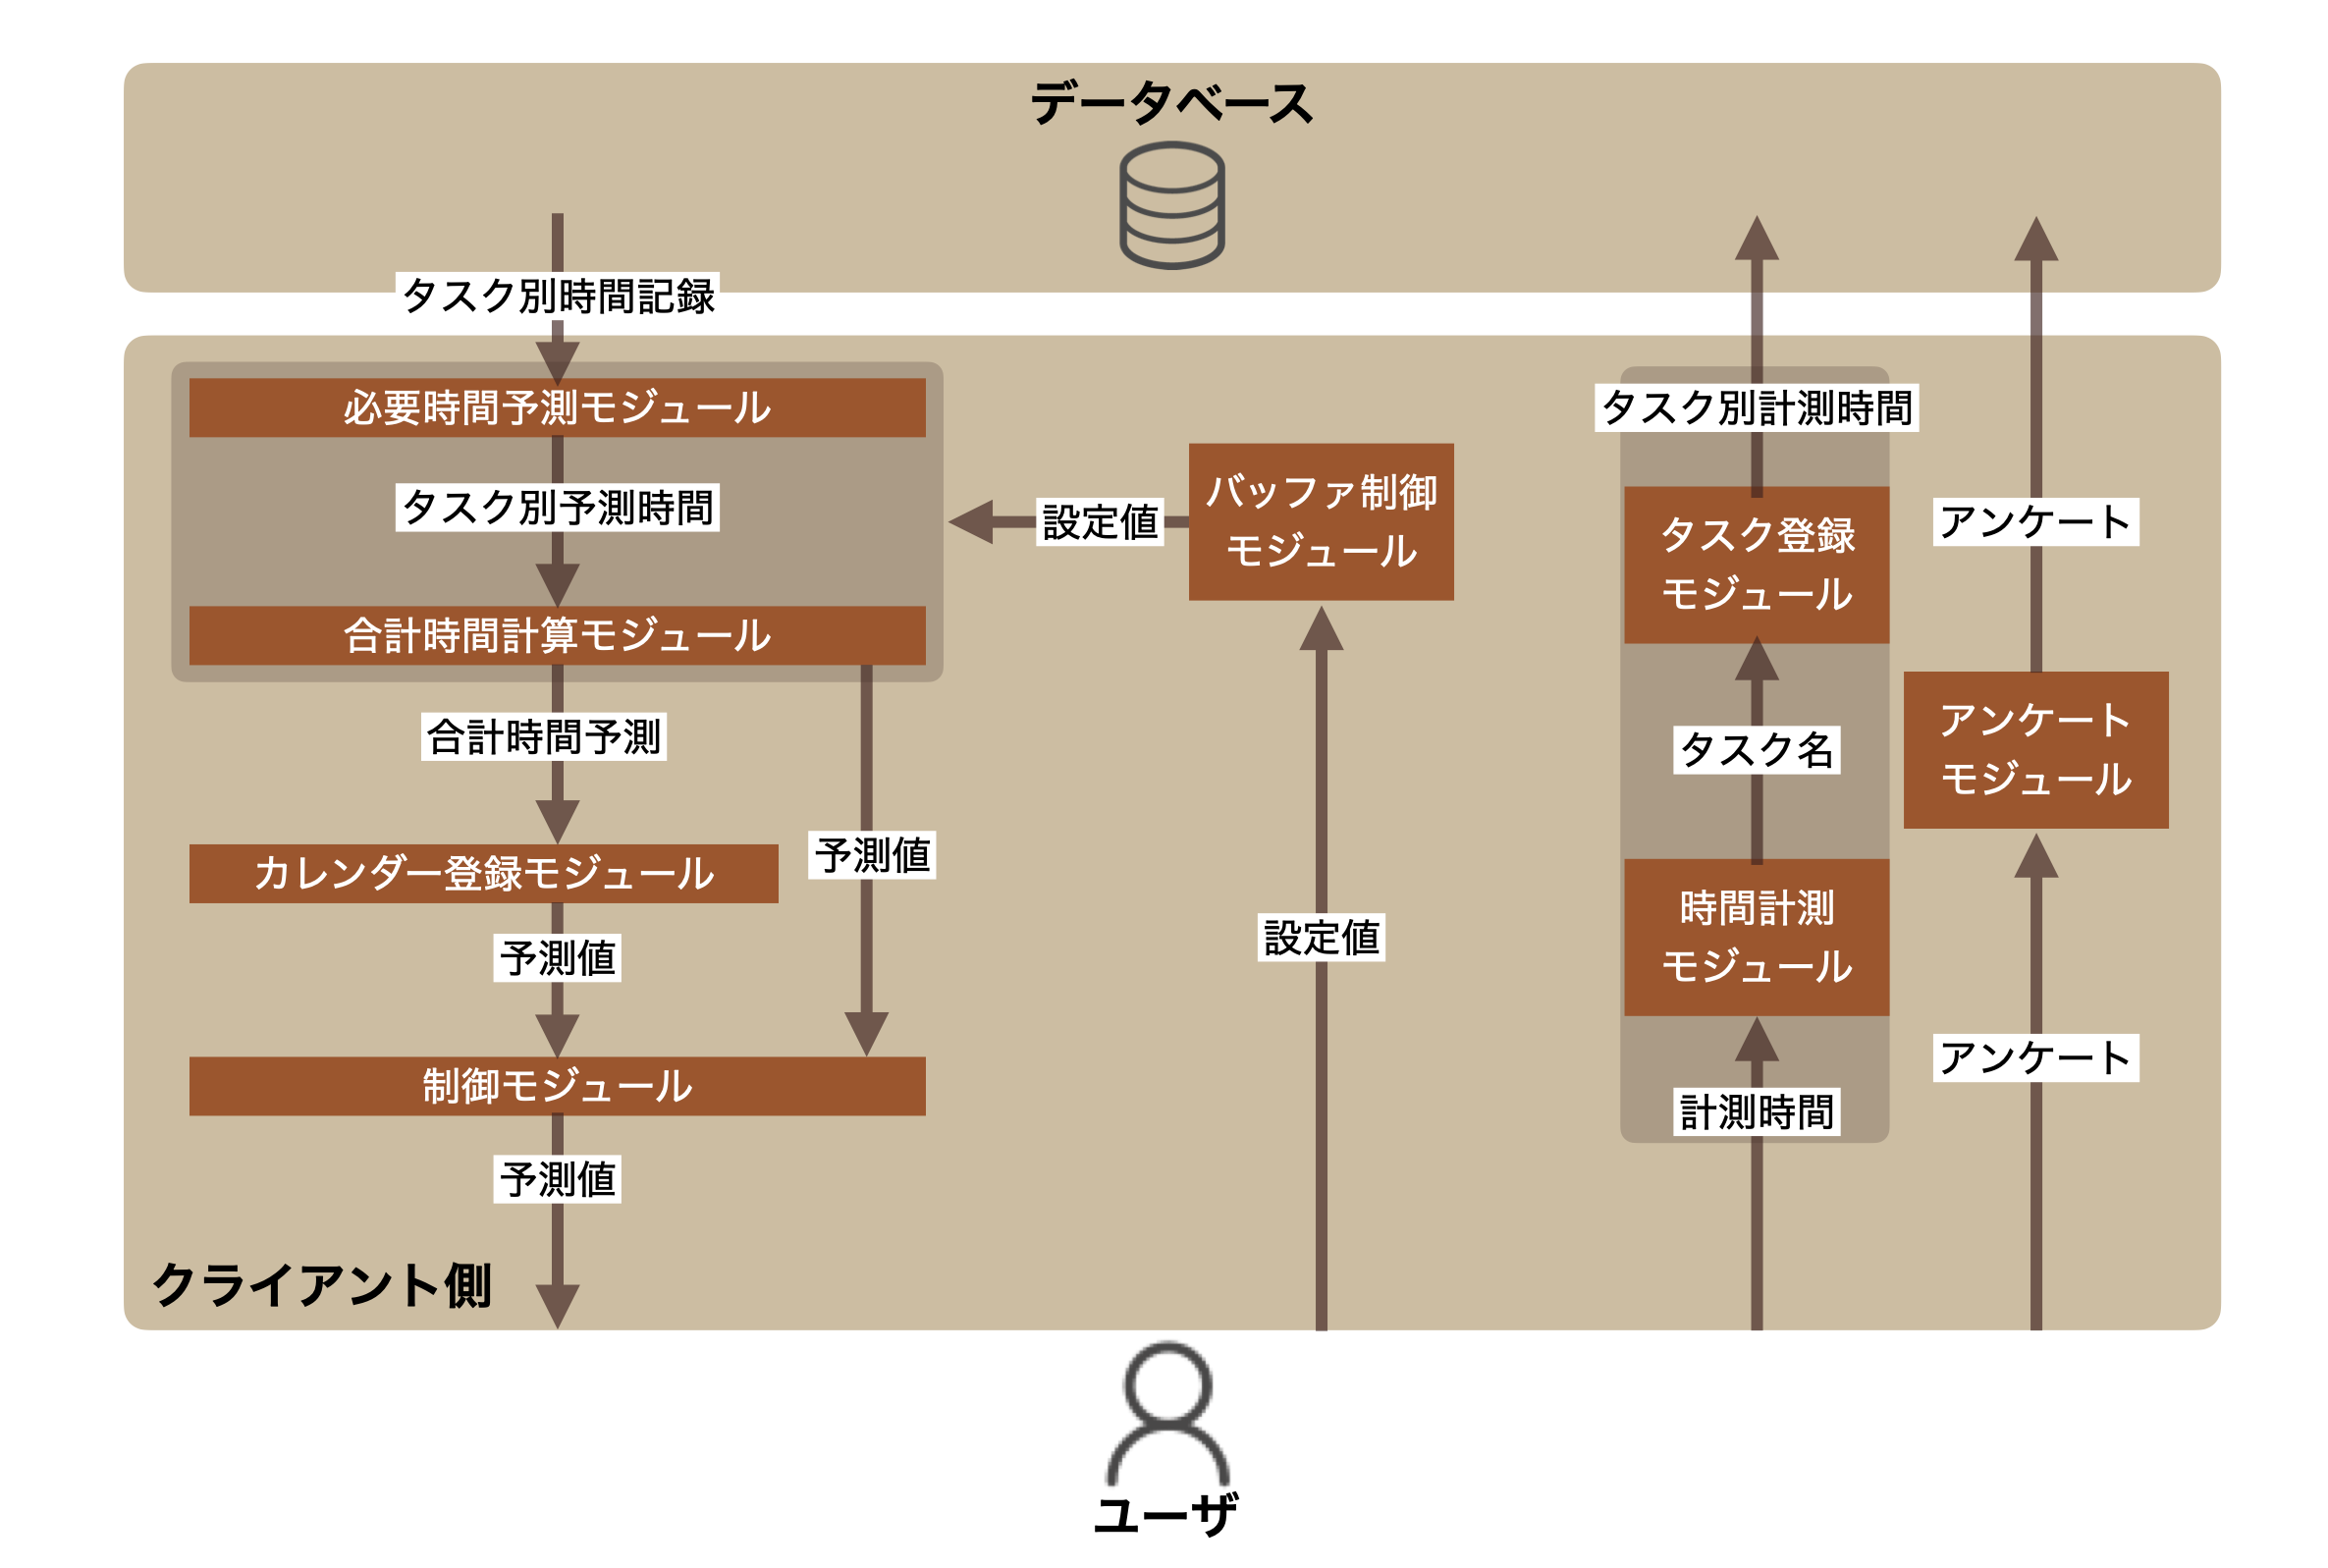
\includegraphics[width=16cm]{images/5/3.png}
	\end{center}
	\caption{システム構成図}
	\label{fig:system}
\end{figure}

\subsection{タスク別時間記録モジュール}
タスク別時間記録モジュールでは,ユーザが行動した時間をタスク別に記録を行う.
ユーザは本システムのストップウォッチを用いて時間を測定する.
時間の測定を終了するとタスク選択画面にて行った行動を選択する.
タスク選択画面には過去入力したタスク名がリスト形式で表示されており,新規タスクである場合は新規タスク名を登録する.

本モジュールはタスク名別に時間を記録し,サーバに送信する.
タスク別時間記録モジュールはユーザが行動したタスク及び時間を記録するモジュールである.
メイン画面のUIButton``TIMER"を押すと,ストップウォッチ画面に遷移する.(図~\ref{fig:stopwatch}参照)
UIButton``START"を押すとUIButtonが``STOP"に書き換えられた後,
上段に配置したUILabel``00:00:00"から “hh:mm:ss”の書式で書き換えられ経過時間が表示される.

\begin{figure}[ht]
\begin{center}
\begin{tabular}{c}

	\begin{minipage}[b]{0.5\linewidth}
	\begin{center}
		\fbox{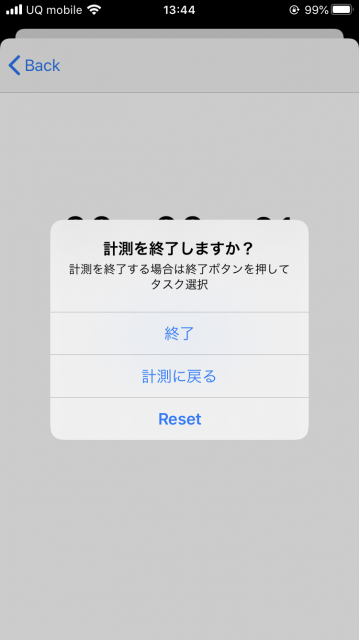
\includegraphics[width=5cm]{images/6/salert.png}}
		\caption{計測に関する選択}
		\label{fig:salert}
	\end{center}
  	\end{minipage}
	
	\begin{minipage}[b]{0.5\linewidth}
	\begin{center}
		\fbox{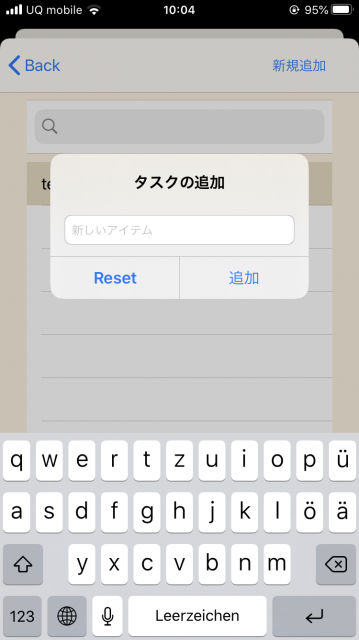
\includegraphics[width=5cm]{images/6/newtask.png}}
		\caption{新規追加}
		\label{fig:newtask}
	\end{center}
  	\end{minipage}
	
	\\
	
	\begin{minipage}[b]{0.5\linewidth}
	\begin{center}
		\fbox{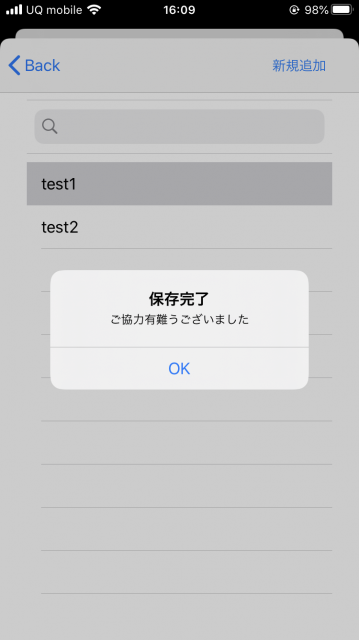
\includegraphics[width=5cm]{images/6/saved.png}}
		\caption{保存完了}
		\label{fig:saved}
	\end{center}
  	\end{minipage}
	
	\begin{minipage}[b]{0.5\linewidth}
	\begin{center}
		\fbox{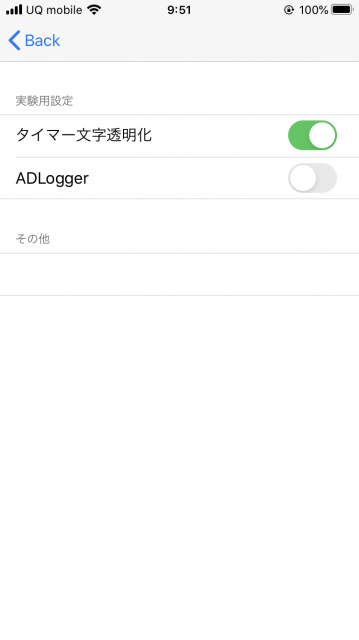
\includegraphics[width=5cm]{images/6/setting.png}}
		\caption{設定画面}
		\label{fig:setting}
	\end{center}
  	\end{minipage}

\end{tabular}
\end{center}
\end{figure}

\begin{figure}[ht]
\begin{center}
\begin{tabular}{c}

	\begin{minipage}[b]{0.5\linewidth}
	\begin{center}
		\fbox{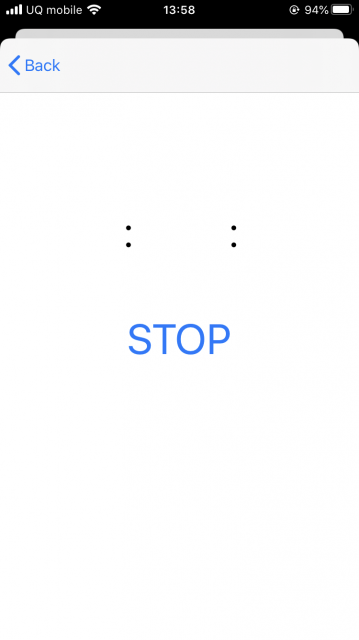
\includegraphics[width=5cm]{images/6/hidden.png}}
		\caption{ストップウォッチ画面の文字透明化}
		\label{fig:hidden}
	\end{center}
  	\end{minipage}

\end{tabular}
\end{center}
\end{figure}


再度UIButtonを押すとタスク別時間記録モジュールによって図~\ref{fig:salert}のようなUIAlertControllerが表示される.
このUIAlertControllerは,``終了"と``計測に戻る"と``Reset"の3つの選択肢を持っている.

``計測に戻る"を選択すると,UIButtonが``STOP"から``START"に書き換えられた後,上記の経過時間測定と同じ方法でカウントアップが再開される.
``Reset"を選択すると,上段の数字はカウントアップを終了しUILabelが``00:00:00"に書き換えられる事でリセット状態となる.
``終了"を選択すると現在のUILabelの値をInt型で変換した後,型で渡し,タスク選択画面へ遷移する.

タスク選択画面ではUITableViewで過去記録した事のあるタスク名が表示される.
各UITableViewCellに表示されているタスク名は,端末内のUserDefaultsにString型の配列として保存されている.
``新規追加"ボタンを押すと,UIAlertControllerが表示される(図~\ref{fig:newtask}).
このUIAlertControllerにはtextFieldが内蔵されており,新規タスクを記入しOKを押すとString型の配列に入力したtextFieldの値が新規タスクとして追加される.
UITableViewCellをタップすると記録した値がサーバーに送信され,保存が成功した事を示すUIAlertControllerが表示される(図~\ref{fig:saved}).
サーバに送られる値は表~\ref{tb:serverdata1}の通りである.尚,ユーザIDはログイン時に端末内のUserDefaultsで保存されたものを送信する.

\begin{table}[htb]
\begin{center}
  \caption{サーバに送信する値}
  \begin{tabular}{|l|l|}\hline
    サーバに送る値 & 型 \\ \hline
    ユーザID & PFUser型(サーバ指定のユーザ型) \\
    タスク名 & String型 \\
    記録時間(秒) & Int型 \\
    記録日時 & Date型 \\
	\hline
  \end{tabular}
  \label{tb:serverdata1}
\end{center}
\end{table}

\subsection{必要時間予測モジュール}
必要時間予測モジュールでは,ユーザの単一タスクないし選択された複数タスクの必要時間を予測する.
``ADLog"ボタンを押し算出画面に移動すると,タスク名毎の予測時間が自動計算されリスト形式で表示される.
リスト内のタスク名を選択すると,中央上段には選択タスクの合計必要時間が自動計算され結果が表示される.
また,同時に中央下段には合計必要時間で追加された合計バッファ時間が内訳として表示される.

メイン画面からUIButton``ADLog"を押すとADLog(必要時間予測)画面に推移される(図~\ref{fig:log}).
ADLog画面のUITableViewでは過去記録した事のあるタスク名とタスク毎の必要時間の予測が表示される.
まず,画面が読み込まれると同時にUserDefaultsに保存した値と一致するユーザIDをサーバで検索する.
該当するデータはタスク名(表~\ref{tb:tasktime_object}のtaskname)をkey,記録時間(表~\ref{tb:tasktime_object}のtasktime)をvalueとするDictionary型の配列を生成する.
valueは更にIntの配列としており,タスク名が重複された場合は記録時間をvalueの配列に追加する.
配列が生成し終わると平均時間$\bar{T}$を算出し,UITableViewCellの左側にタスク名,右側に平均時間$\bar{T}$を表示する.
UITableViewCellをタップすると中央一段目のUILabelを$T_{sum}$(数式(\ref{Ts}))の結果に書き換え,
中央二段目左のUILabelをタスクの$Tv$(数式(\ref{Tv}))の合計に,中央二段目右のUILabelを$Tf$に書き換える.
尚,$Tv$の$N$及び$Tf$は設定画面からのUserDefaultsによって決定される.
またUITableViewCellはaccessoryTypeにcheckmarkが指定されており,UITableViewCellがタップされると右側にチェックマークを表示しユーザが現在どのタスクを選択しているかを示す.

\subsection{カレンダー登録モジュール}
必要時間予測モジュールで算出された合計バッファ時間に関しては,タスク名,予定日時を入力し,
予定日時は開始時刻か終了時刻かの選択を行った上で``追加"ボタンを押すとappleのカレンダーに予定が登録される.

本モジュールはEventKitを用いて必要時間予測モジュールが算出した合計時間をAppleカレンダーに登録する.
カレンダー登録画面を開くと,ユーザが選択したタスクをもとに合計された$T_{sum}$(数式(\ref{Ts}))が受け渡されUILabelに表示される.
また,本モジュールにはカレンダーに登録したいタスク名を入力するUITextField,日時を決めるDatePickerが内蔵されたUIAlertController,DatePickerで選択したデータが開始時刻であるか終了時刻であるか決めるUISegmentedControlが存在する.
すべての項目を入力し,下部のUIButton``追加"を押すとAppleのカレンダーに入力の許可を確認した上で入力した値をカレンダーに渡し登録する事ができる.

\subsection{アンケートモジュール}
アンケートの質問に回答されたタスク名,タスク別所要時間,総合時間をサーバに送信する.
アンケートモジュールには複数のUITextFieldが搭載され,ユーザの入力した下記データをサーバに登録する.
\begin{table}[htb]
\begin{center}
  \caption{サーバに送信する値}
  \begin{tabular}{|l|l|} \hline
    サーバに送る値 & 型 \\ \hline
    ユーザID & PFUser型(サーバ指定のユーザ型) \\
    タスク名 & String型 \\
    タスク予測時間(秒) & Int型 \\
    総合予測時間(秒) & Int型 \\
    記録日時 & Date型 \\
	\hline
  \end{tabular}
  \label{tb:serverdata2}
\end{center}
\end{table}

\subsection{バッファ制御モジュール}
本システムではバッファ制御モジュールを通じてユーザは変動バッファ($Tv$)と固定バッファ($Tf$)を操作できる様にしている.
バッファ制御モジュールは設定画面にて操作が可能である.
変動バッファモードは``変更ボタン"を押すと``急ぎ"・``やや急ぎ"・``ややゆっくり"・``ゆっくり"の4つの選択肢が選べる.
選択肢によって数式(\ref{Tv})の$N$が変動し,必要時間予測モジュールに表示される色が下記の様に変化する(表~\ref{tb:buffer}).
\begin{table}[htb]
  \begin{center}
  \caption{バッファモードの選択分岐}
  \begin{tabular}{|c|c|c|} \hline
    モード & N & 表示色  \\ \hline \hline
    急ぎ & 0 & 赤  \\ \hline
    やや急ぎ & 1 & オレンジ  \\ \hline
    ややゆっくり & 2 & 緑  \\ \hline
    ゆっくり & 3 & 青  \\ \hline
  \end{tabular}
    \label{tb:buffer}
  \end{center}
\end{table}
固定バッファモードは設定画面に直接数字を入力し,``変更"ボタンを押すと入力した値を固定バッファとして計算式に追加する事が可能である.

設定画面はUITableViewで設計されており,2つのUITableViewCellがある.
UITableViewCellにはそれぞれUILabelが設置されており,``変動バッファモード"と``固定バッファ時間"と書かれている.

変動バッファモードのCellにはUIButton``変更"があり,UIButtonを押すとUIAlertControllerが現れる.
UIAlertControllerには``急ぎ"``やや急ぎ"``ややゆっくり"``ゆっくり"の4つの選択ができ,押すとそれぞれ0,1,2,3の値をUserDefaultsに登録できる.

固定バッファモードのCellには3つのUITextField及びUIButton``変更"が搭載されている.
3つのUITextFieldはそれぞれ時間,分,秒の入力を想定しており,入力しUIButton``変更"を押すと秒に変換しUserDefaultsに登録する.


\subsection{表示制御モジュール}
本モジュールは実験の関係上,最初は必要時間予測モジュールを使わず,経過時間を可能な限り閲覧できない環境にする為のものである.
表示制御モジュールは設定画面にて以下の制御が可能である(表~\ref{tb:hyoji}).
\begin{table}[htb]
\begin{center}
  \caption{表示制御モジュールの機能について}
  \begin{tabular}{|l|l|} \hline
   1 & 合計時間の算出画面へのロック機能 \\ \hline
   2 & ストップウォッチの透明化機能 \\ \hline
  \end{tabular}
  \label{tb:hyoji}
\end{center}
\end{table}
合計時間の算出画面へのロック機能は"ADLog"カラムを"OFF"にする事で"ADLog"ボタンから行動記録を見る事の制限をする事ができる.
ストップウォッチの透明化機能は"文字透明化"カラムを"ON"にする事でストップウォッチ作動時に時間経過のカウントアップが非表示となる.
初期設定は"ADLog"カラムを"OFF","文字透明化"カラムを" ON"としている.
いずれも"HELP"ボタンから閲覧できる"設定"ボタンの先にある設定画面からスイッチ形式で操作できる様にした.

設定画面はUITableViewで設計されており,2つのUITableViewCellによって成り立つ.
各UITableViewCellにはUISwitchが搭載されておりタップで操作が可能である.
初期設定は``文字透明化"が``ON",``ADLog"が``OFF"になっている.
``文字透明化"が``ON"だとストップウォッチ画面の経過時間を示すUILbelがhiddenとなり非表示となる(図~\ref{fig:hidden})
``ADLog"が``OFF"だとメイン画面のUIButton"ADLog"が機能せずUIButtonを押してもADLog画面に推移できなくなる.
ユーザがUISwitchを操作するとUserDefaultに保存され,状態が変化する.

\subsection{サーバ側設計}
サーバー側ではユーザ別に登録タスクとタスク時間記録をサーバ内にて管理する.
サーバ及びデータベースには,MBaaSであるBack4App~\cite{back4app}を利用する.
データベースにはユーザの認証情報を格納するUserクラスと, 行動時間記録を格納するtasktimeObject,アンケート 用のsurveyObject,survey2Objectが存在する.
Userクラスの例を表~\ref{tb:user_class},tasktimeObjectの例の例を表~\ref{tb:tasktime_object},surveyObjectの例の例を表~\ref{tb:survey_object},survey2Objectの例の例を表~\ref{tb:survey2_object}に示す.

\begin{table}[htb]
\begin{center}
  \caption{Userクラスの例}
  \begin{tabular}{|l|l|} \hline
  カラム名 & 値 \\ \hline
    objectId & ``2rg6ZJp7GQ" \\
    username & ``testuser" \\
    password & ``testpassword" \\
    ACL & ``2rg6ZJp7GQ" \\
   createdAt & 2020-7-6T07:24:08.810Z  \\
   updatedAt & 2020-7-6T07:24:08.810Z \\ \hline
  \end{tabular}
  \label{tb:user_class}
\end{center}
\end{table}

\begin{figure}[htb]
\begin{center}
\begin{tabular}{c}

\begin{minipage}[htb]{\linewidth}
\begin{center}
  \begin{tabular}{|l|l|} \hline
    カラム名 & 値 \\ \hline
    objectId & ``sRPnWYv0t6" \\
    username & ``testuser" \\
    taskname & ``test1" \\
    tasktiime & 561 \\ 
    createdAt & 2020-7-6T07:24:08.810Z  \\
    updatedAt & 2020-7-6T07:24:08.810Z \\ \hline
  \end{tabular}
   \caption{tasktimeObjectの例}
  \label{tb:tasktime_object}
\end{center}
\end{minipage}

\\

\begin{minipage}[htb]{0.5\linewidth}
\begin{center}
  \caption{surveyObjectの例}
  \begin{tabular}{|l|l|} \hline
    カラム名 & 値 \\ \hline
    objectId & ``9ooWCZj6mp" \\
    username & ``testuser" \\
    taskname & ``test1" \\
    tasktime & 561 \\ 
    createdAt & 2020-7-6T07:24:08.810Z  \\
    updatedAt & 2020-7-6T07:24:08.810Z \\ \hline
  \end{tabular}
  \label{tb:survey_object}
\end{center}
\end{minipage}

\begin{minipage}[htb]{0.5\linewidth}
\begin{center}
  \caption{survey2Objectの例}
  \begin{tabular}{|l|l|} \hline
    カラム名 & 値 \\ \hline
    objectId & ``bPs2GkrlkG" \\
    username & ``testuser" \\
    totaltime & 1320 \\ 
    createdAt & 2020-7-6T07:24:08.810Z  \\
    updatedAt & 2020-7-6T07:24:08.810Z \\ \hline
  \end{tabular}
  \label{tb:survey2_object}
\end{center}
\end{minipage}
\end{tabular}
\end{center}
\end{figure}
\chapter{実装}
本章では,ADLoggerシステムの実装について述べる.
はじめに実装環境について述べ,ついでTODO型タスク記録モジュール,ストップウォッチモジュールについて説明する.

\section{実装環境}
本節では,本システムにおける実装環境について説明する.本システムはiPhoneアプリケーションであり,実装言語にはSwiftを使用している.

\section{クライアント側実装}
クライアントはiPhoneアプリケーションであり,Swiftによって実装した.
TODO型タスク記録モジュール,ストップウォッチモジュールについて説明する.

\subsection{モジュール}

\section{まとめ}
本章では,ADLoggerシステムの実装について述べた.
次章では,本システムで得られたデータから動機づけの向上を評価し,考察について述べる.

\chapter{評価}
複数タスクにかかる所要時間に対し被験者の予測とADLoggerの予測の差異を比較した上で,
ADLogger導入によって,行動・意識の変容が生じるかどうか評価する.
本章ではまず評価概要を説明し,実験結果を示す.最後に,評価実験から得られた結果をもとに考察を行う.

\section{評価実験の概要}
本研究における評価実験の概要を述べる.はじめに,評価実験を行う目的を説明する.
ついで,評価実験を行う手順について説明する.

\subsection{評価の目的}
本研究では,複数タスクにかかる所要時間の予測に関して被験者の予測とADLoggerの予測の差異を比較する事,
ADLogger導入によって,時間管理に対する苦手意識・行動への変化が起こる事を目的としている.

\subsection{実験評価手法}
今回の評価実験では,被験者に時間の長さを教示し,その長さを産生させる時間産生法\cite{Oguro1961}\cite{Tayama2018}を参考にし3回の計測実験を慶應義塾大学の学生男女30名(目標)に対し1ヶ月実施した.
始めに,被験者は事前に各自保持しているiPhoneにADLoggerをインストールして貰う.
インストール後,実験で用いたい日常生活動作を3タスク程度,各タスク所要時間5分から15分程度を決定し,タスク名,タスク毎の必要時間予測,タスクを連続で行った時の必要時間予測をADLoggerのアンケート画面から回答する.後日zoom\cite{zoom}を用いながら実際に行動して貰い実測値を計測する.

その後,被験者自身が実験用に定めた動作3タスク分に関しては被験者は該当するタスクを日常生活で行う度にアプリケーションに計測して貰う.
尚,ADLoggerの設定は初期設定のまま動かさないものとする.
2週間経過後,再びアンケートを回答した上でzoom\cite{zoom}を用いながら実際に行動して貰い計測を行う.

その後,今度はADLoggerの設定を変更しADLogを使用できる状態にしながら更に動作3タスクを2週間程度各自継続的に計測して貰う.
2週間経過後,再びアンケートを回答した上でzoom\cite{zoom}を用いながら実際に行動して貰い計測を行う.

2回目と3回目のアンケート終了後は,日数が経過しないうちにzoom\cite{zoom}を用いて実験者と面会しインタビューを行う.

評価は上記の全3回における実測値およびアンケートで申告した見積もりとのずれの評価,及び心身面の状態変化を比較する.
ずれの評価は反復測定分散分析(Repeated Measured ANOVA)および四分位数を用いてグループを分けた時のそれぞれの変化量を確認する.

心身面の状態変化に関しては下記に記すインタビューに基づき評価する.
インタビューにて質問する項目は付録Aにて記載した.%ストレスの減少も?

\section{評価結果}
〜〜ここからは仮置き〜〜\\
本節では,本システムの導入後時間管理に対し与える影響について,本評価実験で得られた評価結果を示す.
まず,3回の計測における見積もりと実測値のずれはの分布は以下の様になった.(図~\ref{fig:hakohige}参照)

\begin{figure}[hb]
	\begin{center}
	\fbox{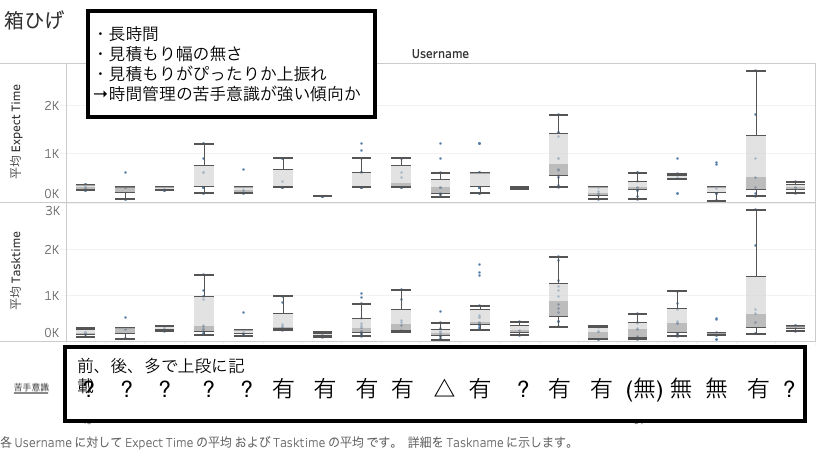
\includegraphics[width=10cm]{images/7/1.png}}
	\caption{3回の計測における見積もりと実測値のずれ(ダミー)}
	\label{fig:hakohige}
	\end{center}
\end{figure}

その上で反復測定分散分析(Repeated Measured ANOVA)を用いて分析したところ,〇〇だった.

また,1回目の計測の結果を元に被験者グループを下記の4つに分類した.(実験結果の四分位数を元に調整)

\begin{table}[htb]
  \begin{center}
  \begin{tabular}{|c|c|c|} \hline
    1 & 大前倒し群 & 予測の方がX分以上長かった群  \\ \hline
    2 & 小前倒し群 & 予測の方がX分未満長かった群  \\ \hline
    3 & 小遅延群 & 実測の方がX分以上長かった群  \\ \hline
    4 & 大遅延群 & 実測の方がX分未満長かった群  \\ \hline 
  \end{tabular}
    \caption{バッファモードの選択分岐}
    \label{tb:buffer}
  \end{center}
\end{table}

その後計測2回分の経過をグループ別に表すとそれぞれ図~\ref{fig:2},~\ref{fig:3},~\ref{fig:4},~\ref{fig:5}の様になった.

\begin{figure}[htb]
\begin{center}
\begin{tabular}{c}

  \begin{minipage}[htb]{\linewidth}
  \begin{center}
  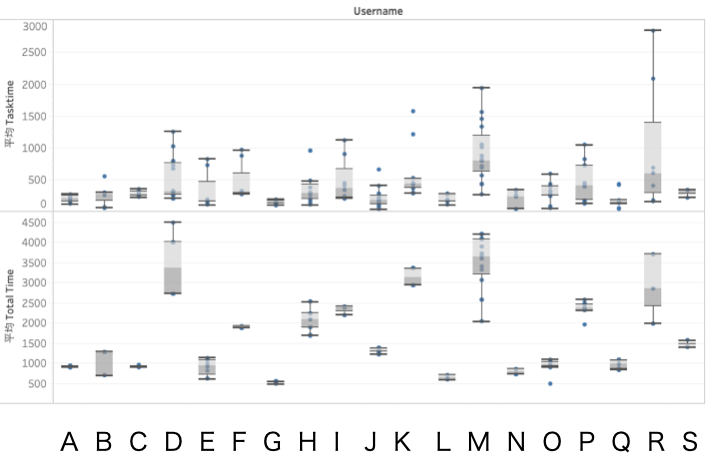
\includegraphics[width=12cm]{images/7/2.png}
  \caption{大前倒し群の推移}
  \label{fig:2}
  \end{center}
  \end{minipage}
  
  \\
  
  \begin{minipage}[htb]{\linewidth}
  \begin{center}
  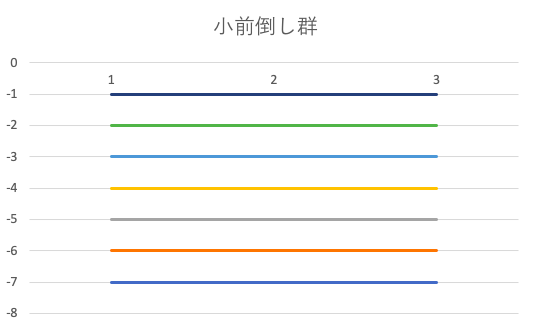
\includegraphics[width=12cm]{images/7/3.png}
  \caption{小前倒し群の推移}
  \label{fig:3}
  \end{center}
  \end{minipage}

\end{tabular}
\end{center}
\end{figure}

\begin{figure}[htb]
\begin{center}
\begin{tabular}{c}

  \begin{minipage}[htb]{\linewidth}
  \begin{center}
  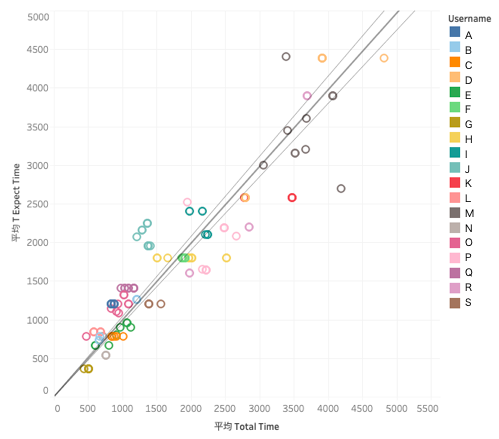
\includegraphics[width=12cm]{images/7/4.png}
  \caption{小遅延群の推移}
  \label{fig:4}
  \end{center}
  \end{minipage}
  
  \\
  
  \begin{minipage}[htb]{\linewidth}
  \begin{center}
  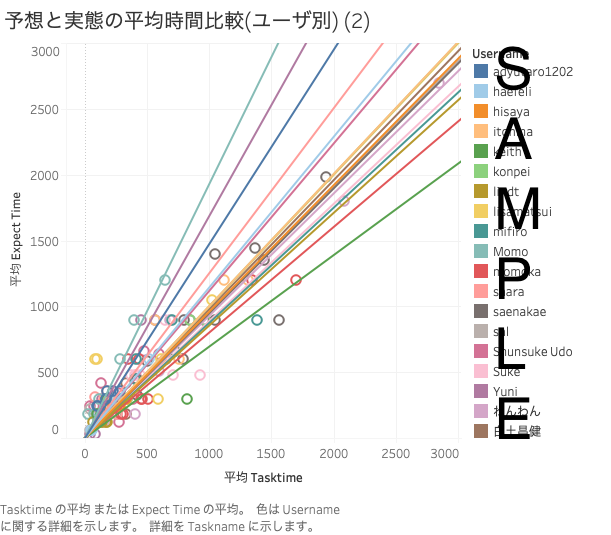
\includegraphics[width=12cm]{images/7/5.png}
  \caption{大遅延群の遷移}
  \label{fig:5}
  \end{center}
  \end{minipage}

\end{tabular}
\end{center}
\end{figure}

\subsection{実験終了後アンケート}

\section{考察}
結果が出次第記述する.

\section{まとめ}
本章では,評価実験にの概要及び手法についてまとめたた上で,結果・考察を述べた.
次章では,本研究における今後の展望と本論文のまとめを述べる.

\chapter{結論}
本章では,本研究における今後の展望と本論文のまとめを述べる.
\section{今後の展望}
本節では,本研究で提案したシステムの問題点と解決策を述べ,今後の展望を述べる.

\subsection{改善点}
今回アプリケーションの介入により被験者によっては予測時間の見積もりが短くなってしまった原因は見積もりの最適化に問題があると考える為,更なる実験でアプリケーションの最適化が必要であると考える.
また,インタビューでは改善すべき点にタイマーを計る過程の効率化や,音声の指示,トラッキングと言った計測の負担を減らす手法やオンオフの差のデータ切り替えのしやすさが提案された為,こうした指摘を元にUI含め改善が必要であると考える.
\subsection{応用例}
本アプリケーションと似た機能を応用すれば朝の準備時間に限らず課題など別のタスクへの応用も可能であると考えられる.
加速度センサーなどを用いた動作検知や機械学習を用いた予測精度の向上が期待できる.
また,ユーザ層への理解を深めることによって時間管理における逆算に関する研究の発展も期待できる.
\section{本論文のまとめ}
本論文では,タスク毎の時間及び合計時間の見積もり精度を向上させるためにADLoggerを提案・実装した.
ADLoggerはトップウォッチで記録されたでタスク毎の時間を基にユーザの行動時間傾向を予測し必要時間見積もりを簡単に導き出せるアプリケーションである.
評価実験は総勢19名の被験者に協力頂き朝の準備支度を想定した環境でADLoggerを使ってもらい評価実験を行った.
結果見積もりの時間と実態の時間のばらつきを縮小させた事が示唆された.
一方で被験者によっては余裕がある予測時間を削る方向で縮小させてしまったり,個人差の大きさなどが問題点として残った.
今後はユーザのタイプに合わせた機能の変化や見積もりの時間の最適化が求められる.
\chapter*{謝辞}

本研究を進めるにあたって,ご指導頂きました慶應義塾大学環境情報学部教授中澤仁博士に深く感謝いたします.
また,慶應義塾大学環境情報学部名誉教授徳田英幸博士,慶應義塾大学大学院政策・メディア研究科特任准教授大越匡博士,慶應義塾大学大学院政策・メディア研究科陳寅特任講師,慶應義塾大学大学院政策・メディア研究科研究員伊藤友隆氏,慶應義塾大学大学院政策・メディア研究科研究員柘植晃氏には,本論文の執筆に当たって御助言を賜りました事を深く感謝致します.
慶應義塾大学中澤研究室の諸先輩方には折りに振れ貴重なご助言を頂きました.
特に慶慶應義塾大学大学院博士課程佐々木航氏,慶慶應義塾大学大学院博士課程礒川直大氏,ダートマス大学博士課程小渕幹夫氏,慶應義塾大学大学院修士課程栄栄元優作氏,慶應義塾大学大学院修士課程片山晋氏には本論文を執筆するにあたってご指導頂きました.
また,慶應義塾大学総合政策学部教授藁谷郁美博士には評価実験にあたりご指導,ご協力をいただきました.
ここに深く感謝の意を表します.

そして,長時間貴重な時間を割いて実験に協力してくれた櫻井怜氏には深く感謝いたします.
陰から研究活動を支えて頂いた,松尾さん,遠藤さんに深く感謝申し上げます.
また,中澤研究室において,柿野優衣氏,川島寛乃氏,谷村朋樹氏,山田佑亮氏,海宝修平氏,鶴岡雅能氏,沼本奨太郎氏,勝又健登氏とは研究活動生活において行動を長く共にし,かけがえのないものとなりました.ここに感謝の意を表します.
最後に,大学4年間に渡る生活を支えてくれた家族に感謝致します.

\begin{flushright}
\today\\
羽柴 彩月
\end{flushright}


\bibliographystyle{unsrt}
\bibliography{bib}

\appendix
\def\thesection{付録\Alph{section}}
\chapter{付録例}
  \section{例1}
\end{document}